%\title{ACTUAL MASTER LAB DOCUMENT}
%This is the original Master Lab Document template, from this the COPY THIS Master Lab Document is created which then can be copied easily to create new labs.
\documentclass{article}
\usepackage[utf8]{inputenc}
\usepackage{cccu_lab}

\modulecode{MCOMD3AOS}
\labtitle{RFC5424 Implementation}
\author{Sebastian Blair}
\date{\today}

\begin{document}
\begin{titlepage}
\makeatletter
\vspace*{5cm}
\begin{center}
\textcolor{Periwinkle}{ % Red font color
		{\Huge \@modulecode}\\[0.5\baselineskip] % Title line 1
		{\Large ---}\\[0.5\baselineskip] % Title line 2
		{\Huge \@labtitle} % Title line 3
}
\end{center}
\rule{\textwidth}{1pt} \\

\begin{center}
\begin{tabular}{r|l}
Author & \textbf{\@author} \\
Last Update & \textbf{\@date} \\
Number of pages & \textbf{\pageref{LastPage}}
\end{tabular}
\end{center}
\centering
\vspace{3em}
\vfill
Environmental Impact Per Page $\approx$ $10.2\unit{L}$ water, $2\unit{g}$ CO$_{2}$ and $2\unit{g}$ wood. 
\vspace{2em}

The environmental effects of paper production include deforestation, the use of enormous amounts of energy and water as well as air pollution and waste problems. Paper accounts for around 26\% of total waste at landfills

\vspace{2em}

Therefore, please print only if this is really necessary.


\end{titlepage}
\makeatother


\section*{Content}
\label{sec:content}

\begin{table}[H]
    \centering
    \begin{tabular}{c|c}
        \nameref{sec:intro} &  \\
         \nameref{sec:get_st}&  \nameref{subsec:func_log}\\
         
    \end{tabular}
\end{table}

\section*{Introduction}
\label{sec:intro}

In this lab you will implement the Internet Engineering Taskforce RFC 5424 standard for syslog using \code{bash}. 

\begin{shaded}
\textbf{\faInfo} \hspace{1em} NOTICE

Be prepared to see a more advanced level of bash scripting through this exercise, as this is a stage 6 module you are expected to learn at higher level. 

Also this lab is essential for the first assignment.
\end{shaded}

Once you have followed this document you will be provided with a file that you can then test the output of the script.

\section*{Getting Started}
\label{sec:get_st}
Open a terminal and make a directory in your \code{\$HOME} directory and call it \code{AOS/} using the \code{mkdir AOS}. 

Next you will need to create a second inside \code{AOS} called \code{logging}. 

From here you can either navigate to this newly created child directory using \code{cd AOS/logging} if you are in the \code{\$HOME} directory still. 

\begin{figure}[H]
    \centering
    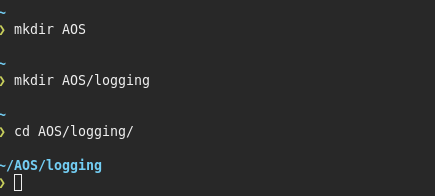
\includegraphics[width=0.5\textwidth]{images/mkdir.png}
    \caption{mkdir example}
\end{figure}

Now pick your favourite text editor(nano, vim, etc) or find an IDE installed on the system. Then create a new shell script like this \code{<editor> rfclogger.sh} where the \code{<editor>} is nano, vim, etc.

At the top we need a sha-bang to point the location of the bash compiler.

\inputminted[frame=single,firstline=1,lastline=4,linenos]{bash}{rfclogger.sh}

This may be the first time you have seen \code{set}, a `BUILTIN'. Essentially, lets you set or unset values of shell options and positional parameters, in this instance we are seting the parameter as \code{-e} which means exit immediately if a command exits with a non-zero status.
\newpage
\begin{shaded}
\textbf{\faSpaceShuttle} \hspace{1em} WANT TO KNOW MORE

You can always view the help or manual page in the terminal command line) by either: 
\begin{itemize}
    \item \code{man <cmd>}
    \item \code{<cmd> <--help || -h >}
    \item For instance \code{set --help}
\end{itemize}
\end{shaded}


\section*{Configurables}
\label{sec:config}

A quick reminder here that \code{\#} is a comment for one line. This bit is essential for running the script but it may help if you come to revisit at a later date.

\inputminted[frame=single,firstline=6,lastline=22,linenos]{bash}{rfclogger.sh}

However, the following code is needed.

\inputminted[frame=single,firstline=23,lastline=34,linenos]{bash}{rfclogger.sh}

A few things to note, 
\begin{itemize}
    \item \code{declare} is a shell BUILTIN that allows the programmer to declare variables and give them attributes. The  option which sets the attribute is \code{-A} and makes the NAMEs associative arrays. Where an associative array variable is used to store multiple data with index and the value of each array element is accessed by the corresponding index value of that element, look at line \code{174} in \nameref{subsec:log_han} section.
    \item All global variables are in UPPERCASE, and as we will see later \code{local} variables are lowercase
    \item \code{export} is a BUILTIN command of the bash shell and other Bourne shell variants. It is used to mark a shell variable for export to child processes.
\end{itemize}

\newpage

\begin{shaded} 
\textbf{\faSpaceShuttle} \hspace{1em} WANT TO KNOW MORE

Experiment with line \code{28} and in a new terminal, (\code{ctrl+t}), type the following:
\begin{itemize}
    \item \code{getent passwd "\$(whoami)"} 
\end{itemize}

What does it return? If you are unsure research to find out what the returned value(s) mean, then do the final part of the command:
\begin{itemize}
    \item \code{getent passwd "\$(whoami)" | cut -d: -f6} 
\end{itemize}

Do you understand how, if not research it?

\end{shaded}
\subsection*{Function for Log Variables}
\label{subsec:func_lv}

We are going to make our first function for this script. 

\inputminted[frame=single,firstline=34,lastline=54,linenos]{bash}{rfclogger.sh}

\begin{itemize}
    \item Bash colours(colors) are implemented when used in conjunction with octal/ANSI escape codes \code{"\textbackslash 033[0;34m"}, see \url{https://www.shellhacks.com/bash-colors/} for further explanation.
    \item If a variable isn't set earlier on or later by some other process of the user bash lets you apply a default value in case of this: So, line \code{39}, if the \code{LOGFILE} is not initialised then \code{LOGFILE:-"\$HOME\/bash-logger.log"} will apply the default log file path location as \code{"\$HOME\/bash-logger.log"}.
    \item Line \code{54}, is how we call a function in a bash script
\end{itemize}

\section*{Individual Log Functions}
\label{sec:indi_lf}
Now we are going to be creating the 8 of the syslog logging levels with an additional 1 to turnoff logging:

\begin{multicols}{2}
    \begin{itemize}
        \item[] \textbf{OFF}
        \item[] DEBUG
        \item[] INFO
        \item[] NOTICE
        \item[] WARNING
        \item[] ERROR
        \item[] CRITICAL
        \item[] ALERT
        \item[] EMERGENCY
    \end{itemize}
\end{multicols}

\inputminted[frame=single,firstline=56,lastline=68,linenos]{bash}{rfclogger.sh}

So again probably some new syntax and commands are standing out. 

\begin{itemize}
    \item \code{"\$FUNCNAMCE"} contains the names of shell functions on the execution call stack, it can store an array of functions.
    \item \code{\$@} expands into a list of separate parameters, where as \code{\$*} is one parameter consisting of all the parameters added together.
    \item Hopefully you remember from other content you have learned at CCCU that \code{exit 0} and is explicit means no error, exit 1 is an error and is implicit. 
\end{itemize}

\section*{Helper Functions}
\label{sec:help_func}

Here the we will have some helper functions to that include the actual log function and level and level name. 

Instead of showing it all in one dump, we will do each one individually. 

\inputminted[frame=single,firstline=73,lastline=87,linenos]{bash}{rfclogger.sh}

So the above code sets out how we want the log format to look like, line \code{74/5} gives an example of usage. Below you can see the output on the terminal when the \code{bash} is passed the \code{-x} option, like debugging.

\begin{figure}[H]
    \centering
    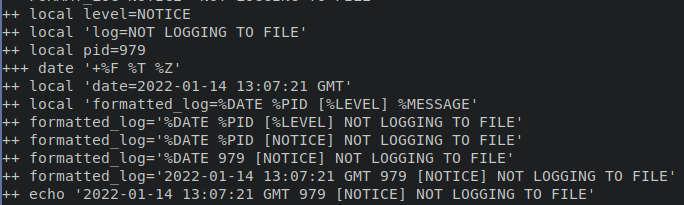
\includegraphics[width=0.9\textwidth]{format_log.png}
    \caption{Format Log function, when called with \code{bash -x \ldots}}
\end{figure}


\inputminted[frame=single,firstline=89,lastline=97,linenos]{bash}{rfclogger.sh}

Only special functionality is the special characters on line \code{95}, \code{\ldots"\$\{level\textasciicircum\textasciicircum\}"} where the caret symbols \code{\textasciicircum\textasciicircum} is shorthand for force to UPPERCASE the value in the variable \code{level}.

\inputminted[frame=single,firstline=99,lastline=105,linenos]{bash}{rfclogger.sh}

Only thing reall to point out here is the that \code{-z} checks to see if something is of length `zero'. The function \code{isset} checks checks whether a variable is set, which means that it has to be declared and is not NULL. Therefore, we can set value by default to \code{LOG\_LEVELS} if the current \code{level} variable is NULL. 

\begin{figure}[H]
    \centering
    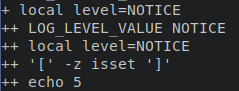
\includegraphics[width=0.4\textwidth]{images/log_level_val.PNG}
    \caption{\code{LOG\_LEVEL\_VALUE} function, when called with \code{bash -x \ldots}}
\end{figure}

\begin{center}
    \vspace{6em}\ldots continued overleaf
\end{center}
\newpage
Next you are going to create function that gets the log name from the supplied numeric value.

\inputminted[frame=single,firstline=107,lastline=116,linenos]{bash}{rfclogger.sh}

\section*{Log Handlers}
\label{subsec:log_han}
We are almost there we a several more functions to write, some that are styling/formatting for colour capable terminals. 

\inputminted[frame=single,firstline=121,lastline=142,linenos]{bash}{rfclogger.sh}

There appears to be a fair amount going on here, but rest assured the structure of the code and commands used therein are pretty much self explanatory. But as always here is an explanation for each key point I sure draw your attention to.

\begin{itemize}
    \item line \code{127}, the \code{-p} is the the flag for pipe and is checking for a piped instance in stdin. A note here \code{/dev/stdin} is unique because it is a symbolic link to \code{/proc/self/fd/0} and \code{/proc/self} is a symbolic link only seen by your running process to its process-id. The \code{/proc} filesystem is a virtual (not real) file system which has the ability to show a different view to each process.
    \item \code{shif} is a BUILTIN command of the Bash shell. When executed, it shifts the positional parameters (such as arguments passed to a bash script) to the left, putting each parameter in a lower position.
    \item line \code{132} checks to see if all arguments are \textbf{not} \code{-n} empty.
\end{itemize}


Below you will see an the output of the \code{if} statement in action. 

\begin{figure}[H]
    \centering
    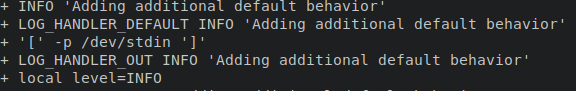
\includegraphics[width=0.7\textwidth]{images/log_handler_defualt_pipe.PNG}
    \caption{\code{LOG\_HANDLER\_DEFAULT} when called using \code{bash -x \ldots} }
\end{figure}

So now we have a function that will handle for colour (color) and non-colour (color) terminals.
You can see that a check is made on line \code{148} where \code{-eq} means equals and it is used for numerical comparison. 

\inputminted[frame=single,firstline=144,lastline=157,linenos]{bash}{rfclogger.sh}

There is also a check for sending the log to a file, line \code{154}.

The below code provides the functionality to match the level of logging to the colours defined correct colour, see \nameref{subsec:func_lv}. 

\inputminted[frame=single,firstline=159,lastline=173,linenos]{bash}{rfclogger.sh}
What we see from the above is that the log message is preceded by a colour and then at the end of the log message colour is returned to default, achieved by line \code{168}.

Furthermore, line \code{170} performs a numerical comparison on the current \code{LOG\_LEVEL} to see if it matches the value OFF(8).

\begin{center}
    \vspace{4em}\ldots continues overleaf
\end{center}
\clearpage

So we have four functions left\ldots

Continuing with the handler theme, the next function is the \code{Log\_HANDLER\_TERM}, essentially the same as the the \code{LOG\_HANDLER\_COLORTERM} but without the colour!

\inputminted[frame=single,firstline=175,lastline=186,linenos]{bash}{rfclogger.sh}

Next function is the deals with the log file itself. Although line \code{192} is not used, it is good to store the argument for future use\ldots

\inputminted[frame=single,firstline=188,lastline=198,linenos]{bash}{rfclogger.sh}

Main things here are the checking if the file exists and if not create it as seen in lines \code{195-196}. Once the file and the message has been logged(line \code{196}) then the system will check to see if a rotation of logs is needed by calling the \code{LOG\_ROTATION} function.

The \code{LOG\_ROTATION} function will rotate the logs every 500 lines, you could modify this to change the value, line \code{204}.

\inputminted[frame=single,firstline=200,lastline=214,linenos]{bash}{rfclogger.sh}

Some explanation will be given for lines \code{203} and \code{206}, the rest is self explanatory.

Line \code{203} counts the number of files in the directory. First \code{ls} is passed the \code{LOGFILE} where only the directory remains \code{\%/*}, then piped \code{|} into grep that the only looks for files that are \code{my-bash-logger.log.\#.gz} where \code{\#} is a number, this intern is piped to \code{wc} and the option \code{-l} will return the number of instances.

Line \code{206}, is a for loop in bash, this is one of several formats, we then decrement the total number of instances of a \ldots*.gz files and then increment the actual file, (rotating).

Lastly, this final function, \code{unsets} all these \code{env} variables when called by the user. 
\inputminted[frame=single,firstline=217,lastline=234,linenos]{bash}{rfclogger.sh}

\begin{shaded} 
\textbf{\faSpaceShuttle} \hspace{1em} WANT TO KNOW MORE

Now that you have been through this document you can use the \code{examples.sh} script to test the functionality of the rfclogger.sh. 

\begin{figure}[H]
    \centering
    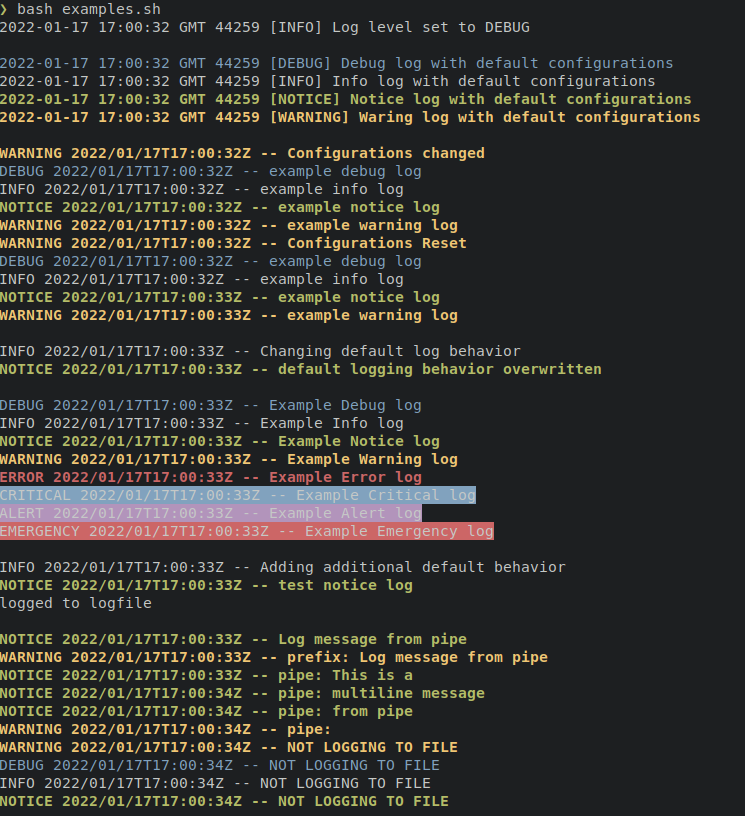
\includegraphics[width=0.6\textwidth]{images/output.PNG}
    \caption{Caption}
\end{figure}
\end{shaded}
\end{document} 
